\chapter{Propuesta}\label{chapter:proposal}
En el presente capítulo se explica la solución al problema fundamental de este trabajo. Se propone la creación de una fabric-chaincode-api que permita la implementación de contratos inteligentes en el lenguaje $ C\sharp $.

La sección $ 2.1 $ aborda las herramientas que facilitan la conexión entre el chaincode y el nodo peer en el lenguaje $ C\sharp $.

En $ 2.2 $ se trata la solución al problema del procesamiento concurrente de transacciones.

En $ 2.3  $se explica la comunicación con el peer para las consultas al ledger.

\section{gRPC y \textit{protocol buffers}}

El chaincode se ejecuta en un entorno desacoplado al resto del nodo \textit{peer}. De esta forma, el \textit{peer} es independiente del lenguaje real en el que se implementa el chaincode. Para cumplir el propósito de este trabajo es necesario implementar el chaincode en $ C\sharp$, lenguaje distinto al del nodo peer (Go). En esta sección se explica gRPC [\cite{grpc-doc}], herramienta que permite la comunicación entre ambos. 

GRPC son las siglas que definen a un \textit{framework} desarrollado por Google sobre Llamada a Procedimiento Remoto (Remote Procedure Call, RPC por sus siglas en inglés). En gRPC, una aplicación cliente puede llamar directamente a un método en una aplicación servidor en una máquina diferente como si fuera un objeto local, lo que facilita la creación de aplicaciones y servicios distribuidos. 

Como en muchos sistemas RPC, gRPC se basa en la idea de definir un servicio, especificando los métodos que se pueden llamar de forma remota con sus parámetros y tipos de devolución. En el lado del servidor, se implementa una interfaz para manejar las llamadas de los clientes. En el lado del cliente, se tiene un \textit{stub} que proporciona los mismos métodos que el servidor.

La diferencia con otros frameworks RPC existentes es que gRPC usa \textit{protocol buffers} [\cite{protobuf-doc}] como lenguaje de definición de interfaz para la serialización y como formato de intercambio de mensajes en lugar de JSON/XML.

Los \textit{protocol buffers} proporcionan un mecanismo extensible, independiente del idioma y de la plataforma, para serializar datos estructurados de manera compatible con versiones anteriores y posteriores. Se pueden ampliar con nueva información sin invalidar los datos existentes ni requerir que se actualice el código.

\begin{figure}[tbph]
\centering
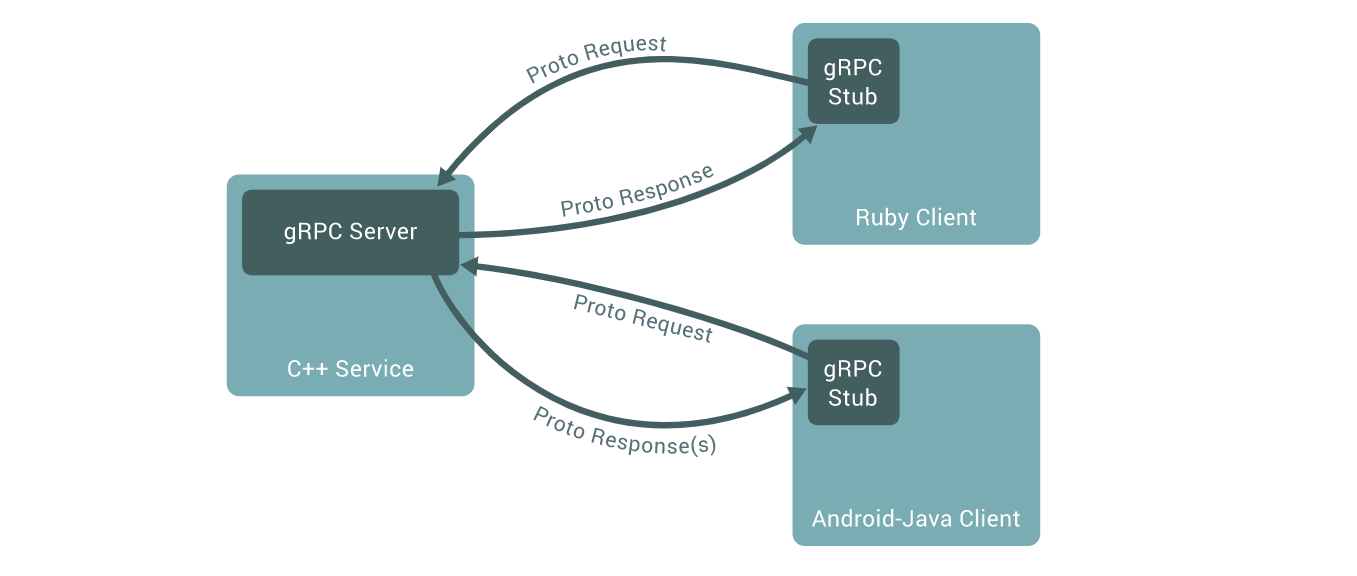
\includegraphics[width=\textwidth]{Images/grpc}
\caption{ Ejemplo de servidor C++ con clientes Ruby y Java.}
\label{fig:grpc}
\end{figure}

Los clientes y servidores de gRPC pueden ejecutarse y comunicarse entre sí en una variedad de entornos y pueden escribirse en cualquiera de los idiomas compatibles con gRPC. En la solución propuesta en este artículo se aprovecha dicha característica para comunicar al nodo \textit{peer} con el chaincode, escritos en Go y $ C\sharp$ respectivamente.

\section{fabric-protos-csharp}
Como se vio en el capítulo anterior, la interacción entre el chaincode y el nodo peer se establece mediante mensajes \textit{protobuf}. El servicio gRPC y las definiciones de \textit{protocol buffers} que se utilizan en Hyperledger Fabric se encuentran en el repositorio \textit{fabric-protos}, de dominio público. Se empleó la herramienta \texttt{protoc} para compilar estas definiciones al lenguaje C$\sharp$. De esa manera se crean las clases bases necesarias para interactuar con Fabric.

%\section{getChannelId}
%\section{getTxTimeStamp}
%\section{getCreator}
%\section{createCompositeKey}
%\section{splitCompositeKey}
%\section{getState}
%\section{putState}
%\section{deleteState}